\chapter{Design and implentation}
The market app should be easy to use and fit for consumers of all ages. To install an application the user has to select a desired application with one touch, then check the specification if its compatible with the Arduino, then a agree/install button for installing the app on the Arduino. This is a total of two clicks, despite you have chosen a category or search hits on the market app. This is similar to Google Play.\\
\newline
Each (supported) Arduino device is equipped with a Unified Resource Identifier (URI) stored in its ROM. This URI is automatically transferred to the market app once it is turned on and is in range; the hardware configuration (Memory, connected devices) is stored in a XML file the URI links to.
The app store client can then compare compatibility with the device and app requirements.
Only apps supported on your Arduino will initially be visible in the market application, however, power users can enable unfiltered results to browse the selection and consider upgrading the device.\\
\newline
Anyone modifying a board will have to provide a hardware specification and transfer a new URI to the device if they want filtered results in the app store (Such a user could still choose to view and install unfiltered applications).
The URI could also be read from a QR-code.

\subsection{System Architecture}
	The design was divided into several modules:
	\begin{itemize}
		\item{Bluetooth connection between the Android and the Arduino}
		\item{Synchronization with the local SQLite database}
		\item{Android application view (the visible design)}
		\item{A service that contains the protocol for installing ``over the air''}
	\end{itemize}
	\vspace{0.2in}
	
	The system design was implemented such that further developing and extension should be as modular and easy as possible.
	Therefor it is designed as a plugin-like system where you easily can implement your own protocols against a desired device, e.g Raspberry Pi. The application only support STK500 protocol and therefore only connection towards Arduino.
	The design for the connection to other devices are done as following:\\

	\begin{figure}[H]
	\centering
	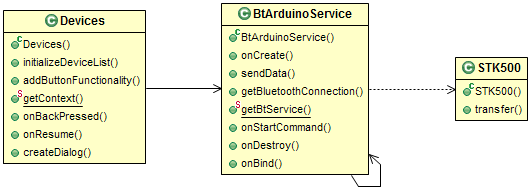
\includegraphics[width=130mm]{images/BTConnection.png}
	\end{figure}

	Devices.java is an Activity and can therefore be considered as a view in the application. To add a new service there is few changes to be done in Devices.java. Afterall an own service and a protocol towards a desired device must be implemented. Since this project only take in hand a connection between Android and Arduino, we implemented the STK500 protocol.
	The overall design solution for multiple connections will be like this:\\

	\begin{figure}[H]
	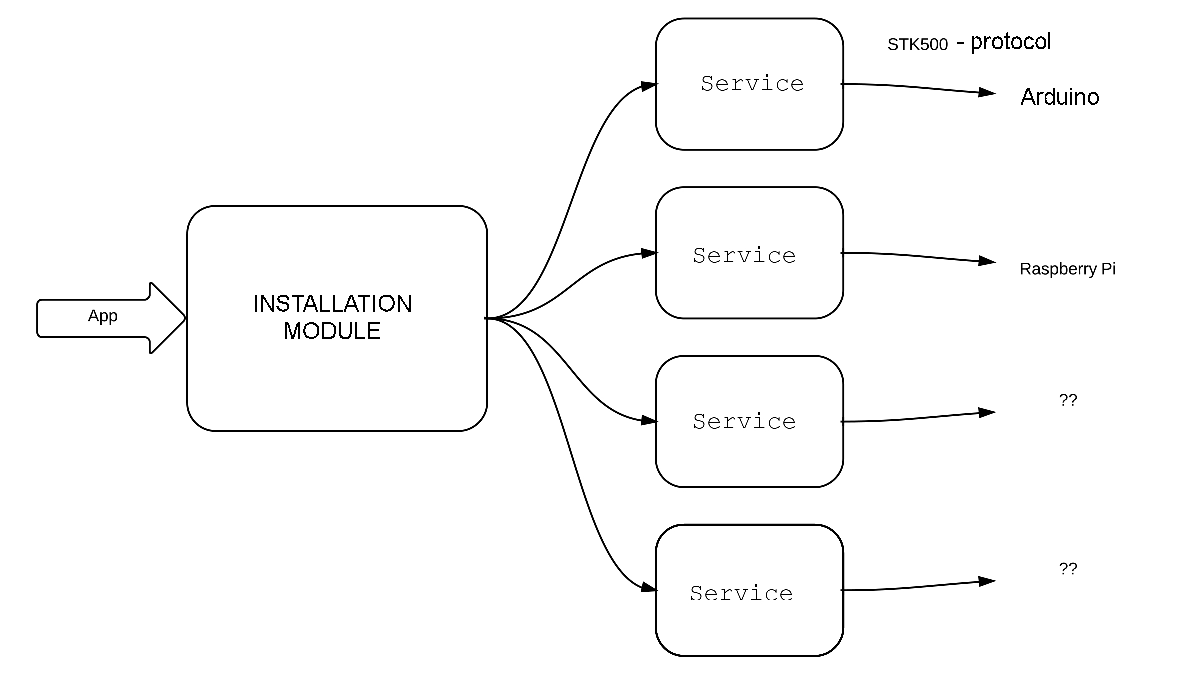
\includegraphics[scale=0.7]{figures/OTAArchitecture.pdf}
	\captionof{figure}{Over The Air Architecture}
	\end{figure}
